\section{Auswertung}
\subsection{Vorverstärkte Pulse auf dem Oszilloskop}
Die Pulse des Surface-Barrier Detektors werden vorverstärkt und einmal mit und einmal ohne Amplifier auf dem Oszilloskop dargestellt.
In den Abbildungen \ref{fig:2} und \ref{fig:1} werden die Pulse gegen die Zeit aufgetragen.

\begin{figure}[H]
  \centering
  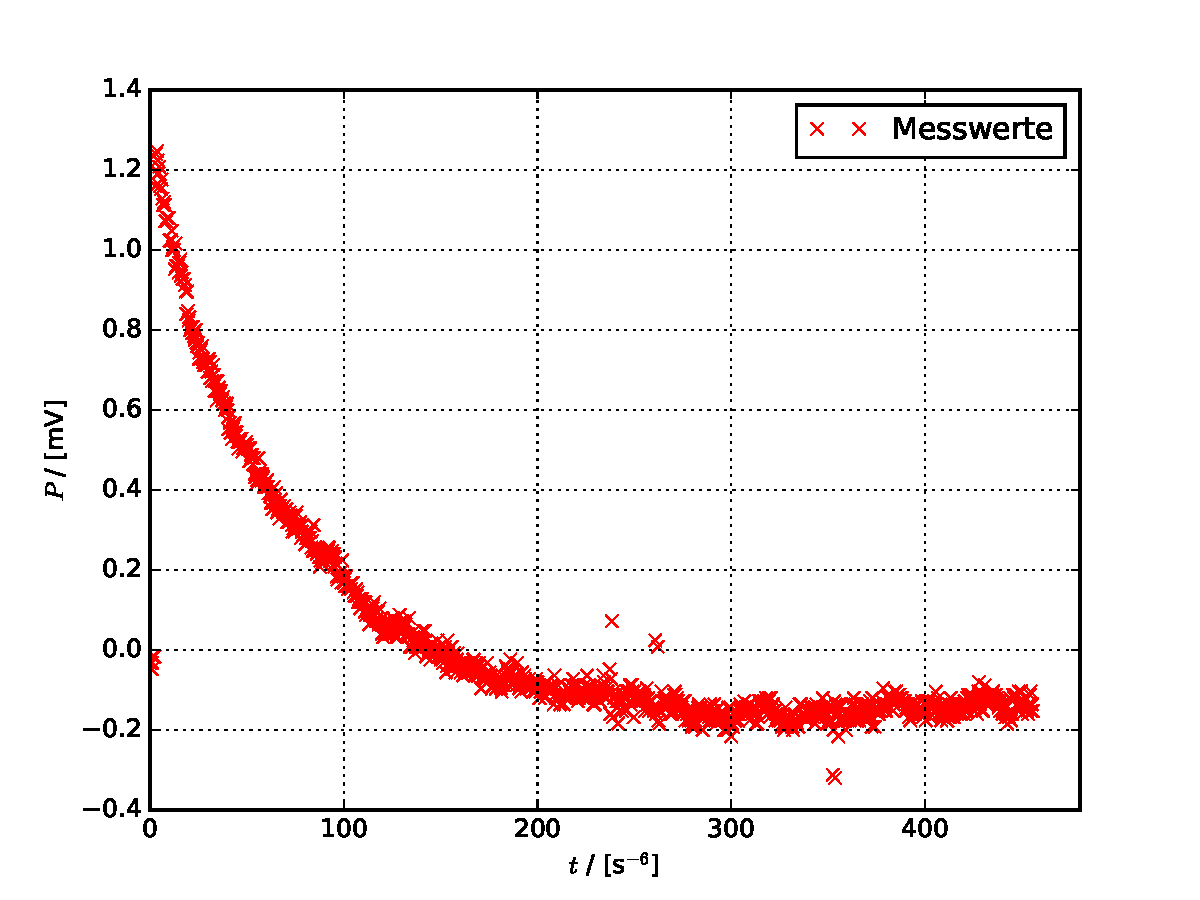
\includegraphics[width=\textwidth]{osz2.pdf}
  \caption{Pulse in Abhängigkeit von der Zeit ohne angeschlossenem Amplifier.}
  \label{fig:2}
\end{figure}

Ohne angeschlosseem Amplifier schwankt der Wert vor dem Puls um $0\,\text{V}$.
Danach steigt der Puls mit einer Anstiegszeit von $0\,\si{\micro\second}$ auf ca. $1,25\,\text{mV}$.
Mit einem "Überschwinger" pendelt sich der Wert wieder auf ca. $0\,\text{V}$ ein.

\begin{figure}[H]
  \centering
  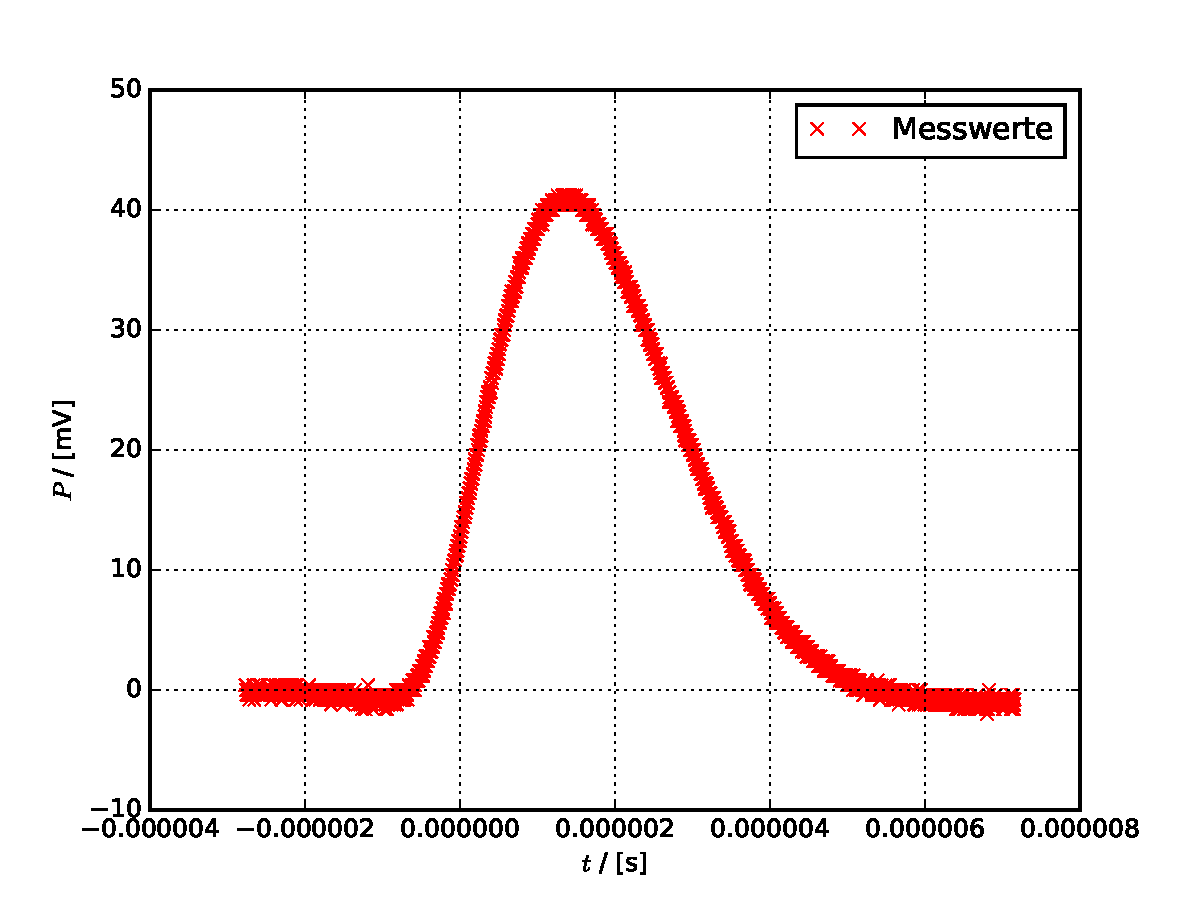
\includegraphics[width=\textwidth]{osz1.pdf}
  \caption{Pulse in Abhängigkeit von der Zeit mit angeschlossenem Amplifier.}
  \label{fig:1}
\end{figure}

Die Anstiegszeit mit angeschlossenem Amplifier beträgt ca. $8\,\si{\micro\second}$.
Der Puls steigt von $0\,\text{mV}$ auf ca. $41\,\text{mV}$ und fällt wieder auf seinen Ursprungswert ab.

\subsection{Bestimmung der Goldfoliendicke}


\subsection{Bestimmung des differentiellen Wirkungsquerschnitts}

\subsection{Untersuchung des Einflusses der Mehrfachstreuung}

\subsection{Messung der Z-Abhängigkeit an einer }
